\section{Execution Flow}
\label{design:flow}

Until now, we have established how the bootware can be called from outside components using a web service interface to start the bootstrapping process.
We also established that big parts of this process will be implemented as plugins.
Now, it is time to take a look at the actual internal structure of the bootware.
What follows is a step by step description of the internal process during a bootstrapping operation.

\begin{figure}[!htbp]
	\centering
	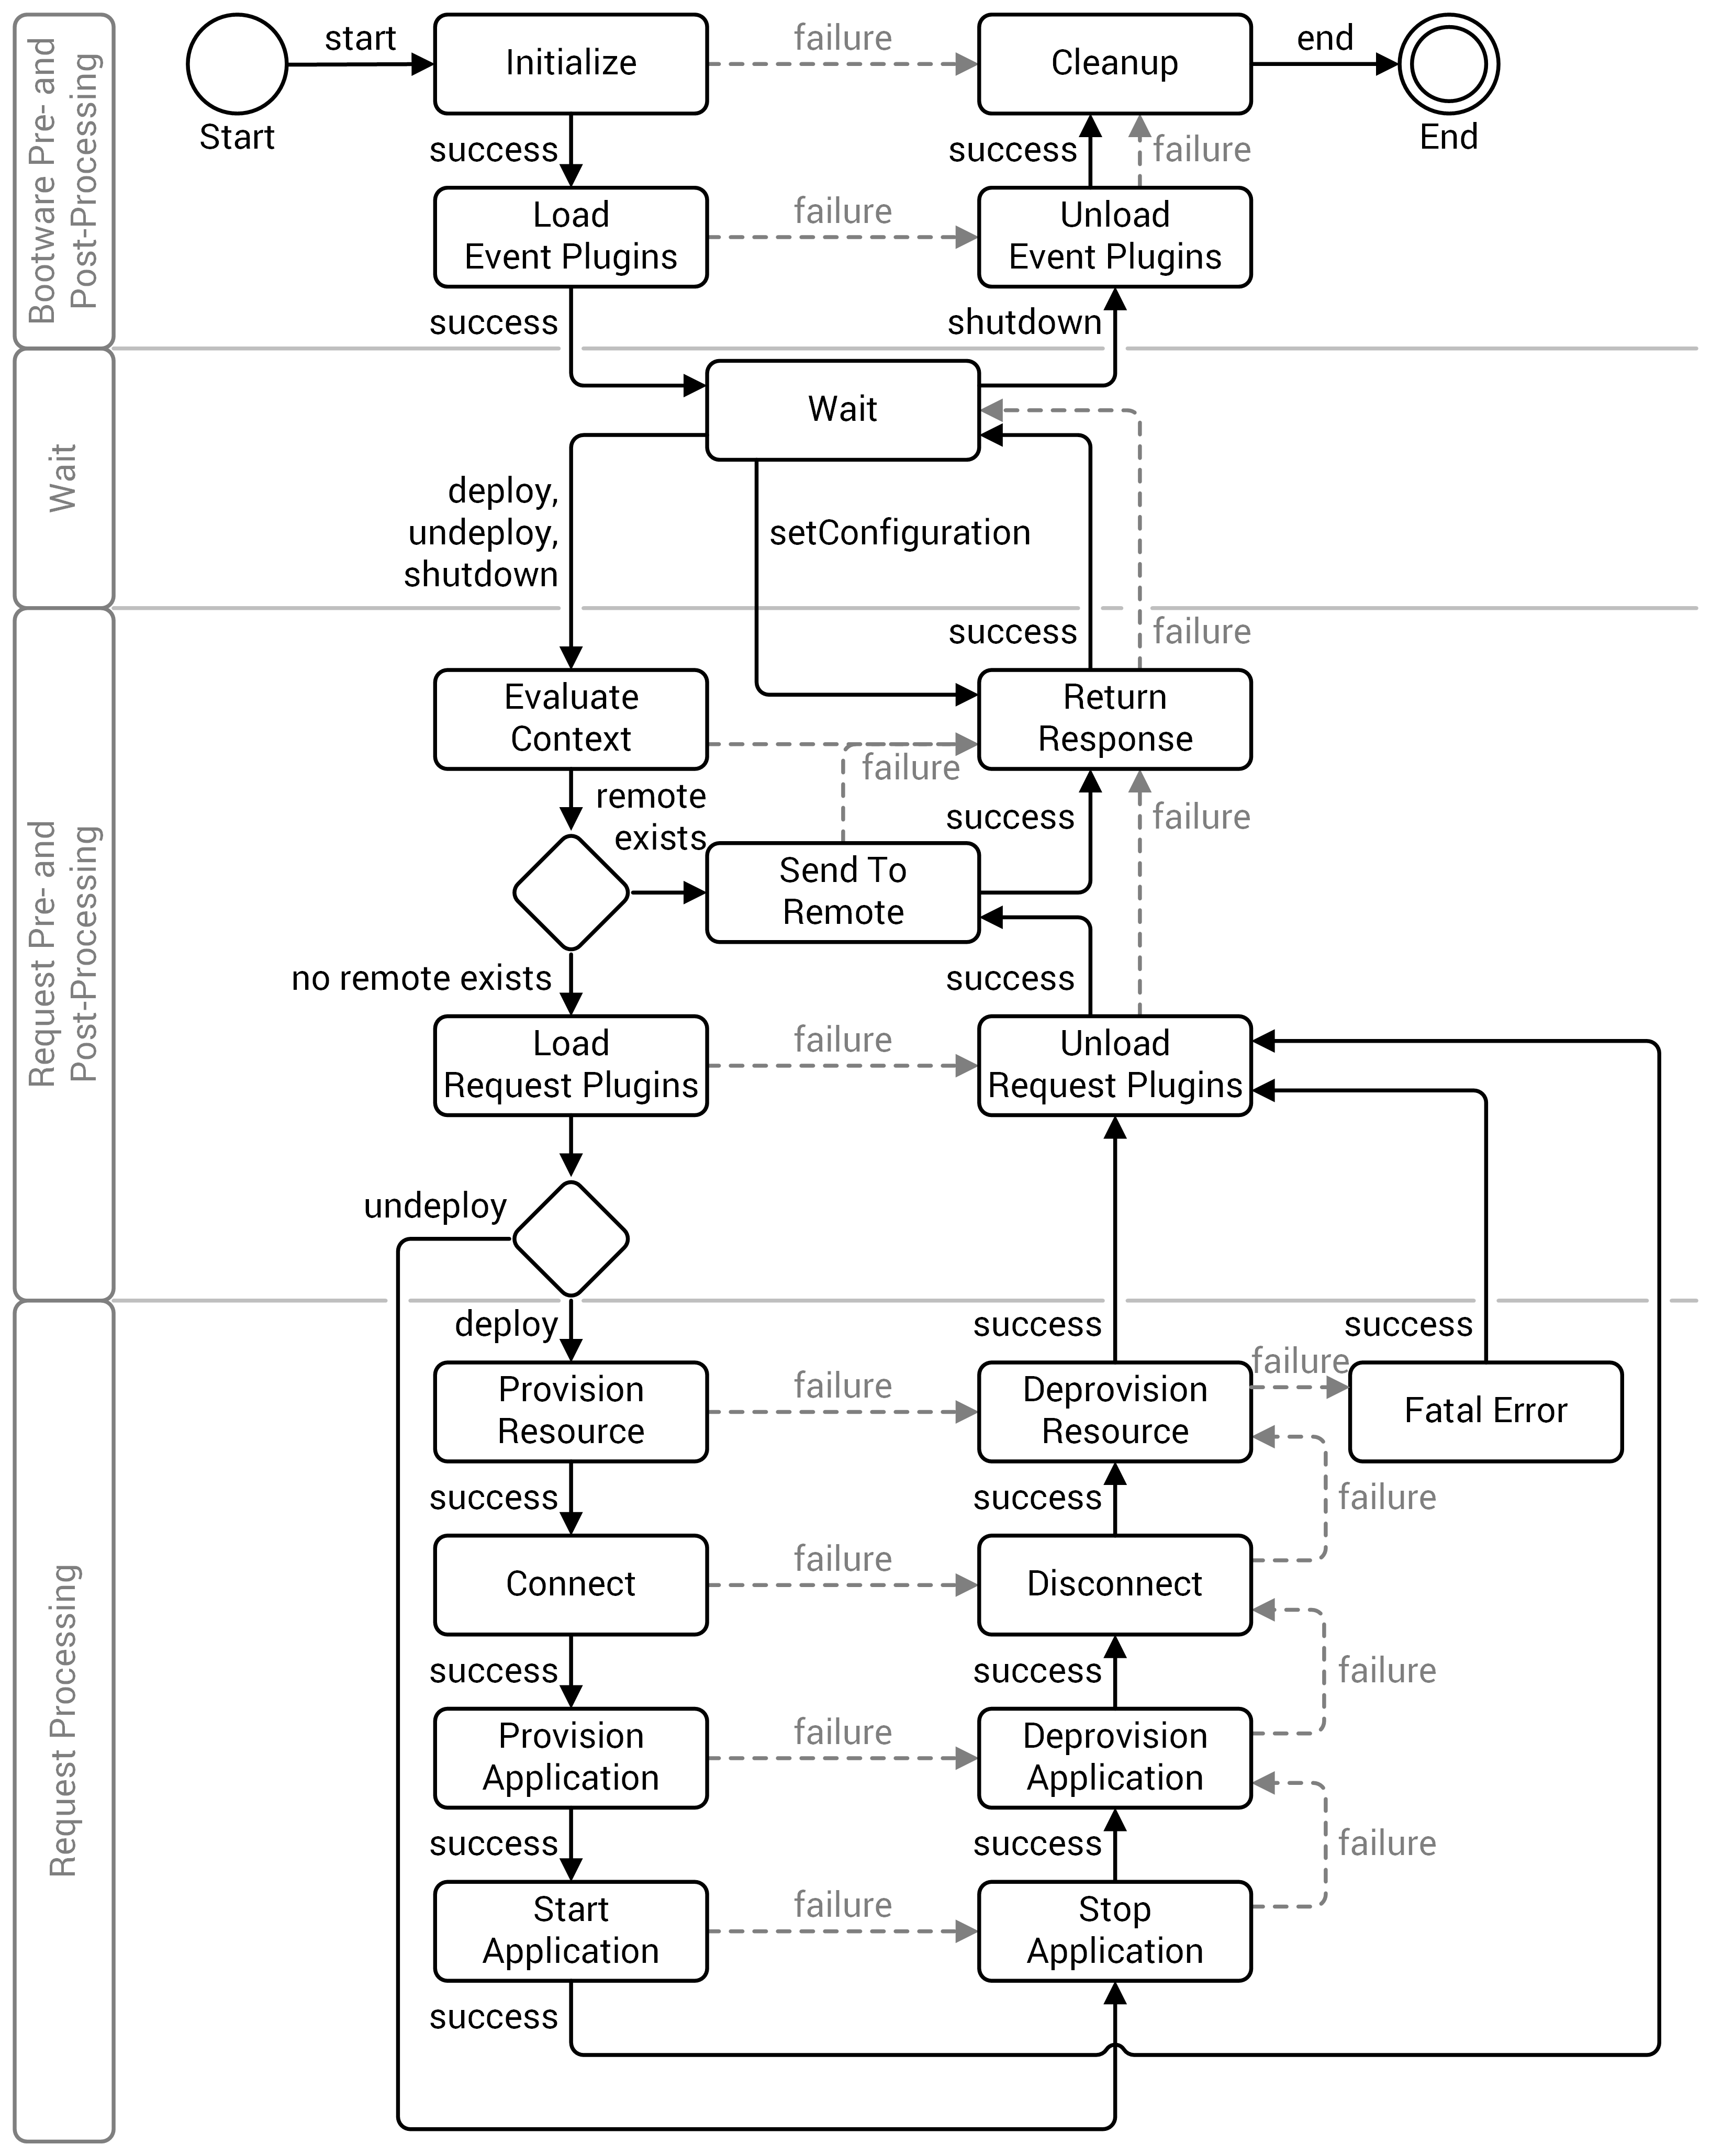
\includegraphics[resolution=600]{design/assets/flow_local}
	\caption{Execution flow in the local bootware.}
	\label{image:flow_local}
\end{figure}

\autoref{image:flow_local} shows a graph that represents the major steps during the bootware execution in the local bootware as flow diagram.
The bootstrapping process is started when the bootware adapter starts the local bootware, which is represented by the \textit{start} activity in the top left corner of \autoref{image:flow_local}.
From there, the bootware first does some initializations.
If those fail for some reason, the cleanup code will be executed before the local bootware execution is ended, as can be seen on the top right corner of \autoref{image:flow_local}.
In most cases however, the initialization should succeed.
Then, the local bootware will execute the next activity, where it tries to load the event plugins.

The event plugins are loaded once at the beginning of the local bootware execution because they will not change at a per request basis (like the other plugins).
Any events generated by the bootware core or by plugins after this point can now be handled by the event plugins.
If loading one of these plugins fails, the local bootware will try to unload already loaded plugins before continuing with the \textit{cleanup} activity.
If the plugins are loaded successfully, the local bootware transitions into the \textit{wait} activity, shown in the top center of \autoref{image:flow_local}.

The local bootware is now ready and waits for requests from the outside.
A deploy request will be send to the local bootware when the bootware adapter calls it to provision the workflow middleware.
A setConfiguration request might also be send by the bootware adapter to set the default configuration.
The undeploy and shutdown request will be triggered by the local bootware itself, when it is time to deprovision the workflow middleware and the remote bootware.

If a shutdown event is received, the local bootware will first tell the remote bootware to undeploy all active applications.
Next, the local bootware will undeploy the remote bootware by running through the undeploy process fragment shown on the bottom left with the appropriate plugins.
Then, it will shut itself down by first unloading the event plugins and then running the cleanup code.
This is the only normal way to shut down the bootware.
We only hint at the setConfiguration request here, since it just replaces the saved configuration with the one sent in the request.
Deploy and undeploy requests however are more complicated.
If such a request is received, the local bootware transitions to the next activity, where it evaluates the request context.

In the \textit{evaluate context} activity, the information send with the request is used to generate the full context, which contains all the information necessary to fulfill the request, as described in \autoref{design:context}.
If this cannot be done for some reason, the local bootware returns a response containing an error message before returning to the \textit{wait} activity.
If the context is created successfully, the local bootware tries to send the request on to the remote bootware, as shown in the middle of \autoref{image:flow_local}.
For this to work, the remote bootware has to exist in the requested remote environment, which will not be the case during the first execution.
Therefore, the local bootware first has to provision the remote bootware in the requested remote environment and so it transitions to the \textit{load request plugins} activity.
In the \textit{load request plugins} activity the plugins specified in the context are loaded.
If this fails, the local bootware tries to unload already loaded plugins before returning an error response and returns to the \textit{wait} activity.
If the plugins are loaded successfully, the local bootware now starts either the deploy process fragment at the bottom left, or the undeploy process fragment shown at the bottom right of \autoref{image:flow_local}, depending on the type of the request.

If the request was a deploy request, the local bootware will now execute the steps shown in the bottom left of \autoref{image:flow_local} one after another.
In the \textit{provision resource} activity, the deploy operation of the resource plugin will be called.
Then, in the \textit{connect} activity, a connection with this resource will be established by the communication plugin.
Over this connection, the requested application is provisioned in the \textit{provision application} activity, and started in the \textit{start application} activity, using the application plugin.
If one of these activities fails, the local bootware transitions over to the corresponding undeploy activities on the right and works its way backwards to undo all operations that where already executed.
This process fragment is the same as the undeploy process, shown on the bottom right of \autoref{image:flow_local}, which is triggered by an undeploy request.

If the \textit{stop application}, \textit{deprovision application}, or \textit{disconnect} activities fail, the local bootware just continues with the next undeploy activity because these operations are not considered critical.
However, if the \textit{deprovision resource} activity fails, the local bootware transitions to a \textit{fatal error} activity, shown at the right of \autoref{image:flow_local}, because this step is considered critical.
This activity failing could mean that resources are still active in the cloud and human interaction is necessary to remove them to stop further costs from incurring.
The \textit{fatal error} activity is responsible for taking special actions to remedy this situation.
The successful, as well as the unsuccessful execution of either the deploy or the undeploy process all finish with the \textit{unload request plugins} activity, where the plugins that where needed for this particular request are unloaded.
If everything went as planned, a remote bootware should now be running in the desired cloud environment and the local bootware can now pass on the request to this remote bootware, as shown in the center of \autoref{image:flow_local} with the \textit{send to remote} activity.
The local bootware will wait here until it receives a response from the remote bootware.

Now, we move our attention to the remote bootware, where the requests continues to be processed.
\autoref{image:flow_remote} shows the execution flow of the remote bootware.
As we can see, it is largely identical to the local bootware.
The \textit{send to remote} activity is gone because it is not needed in the remote bootware.
Instead, as the bottom of \autoref{image:flow_remote} shows, the \textit{provision middleware} and \textit{deprovision middleware} activities were added.
The remote bootware also supports the getActiveApplications request.
Other than that, the local and remote processes are the same.

\begin{figure}[!htbp]
	\centering
	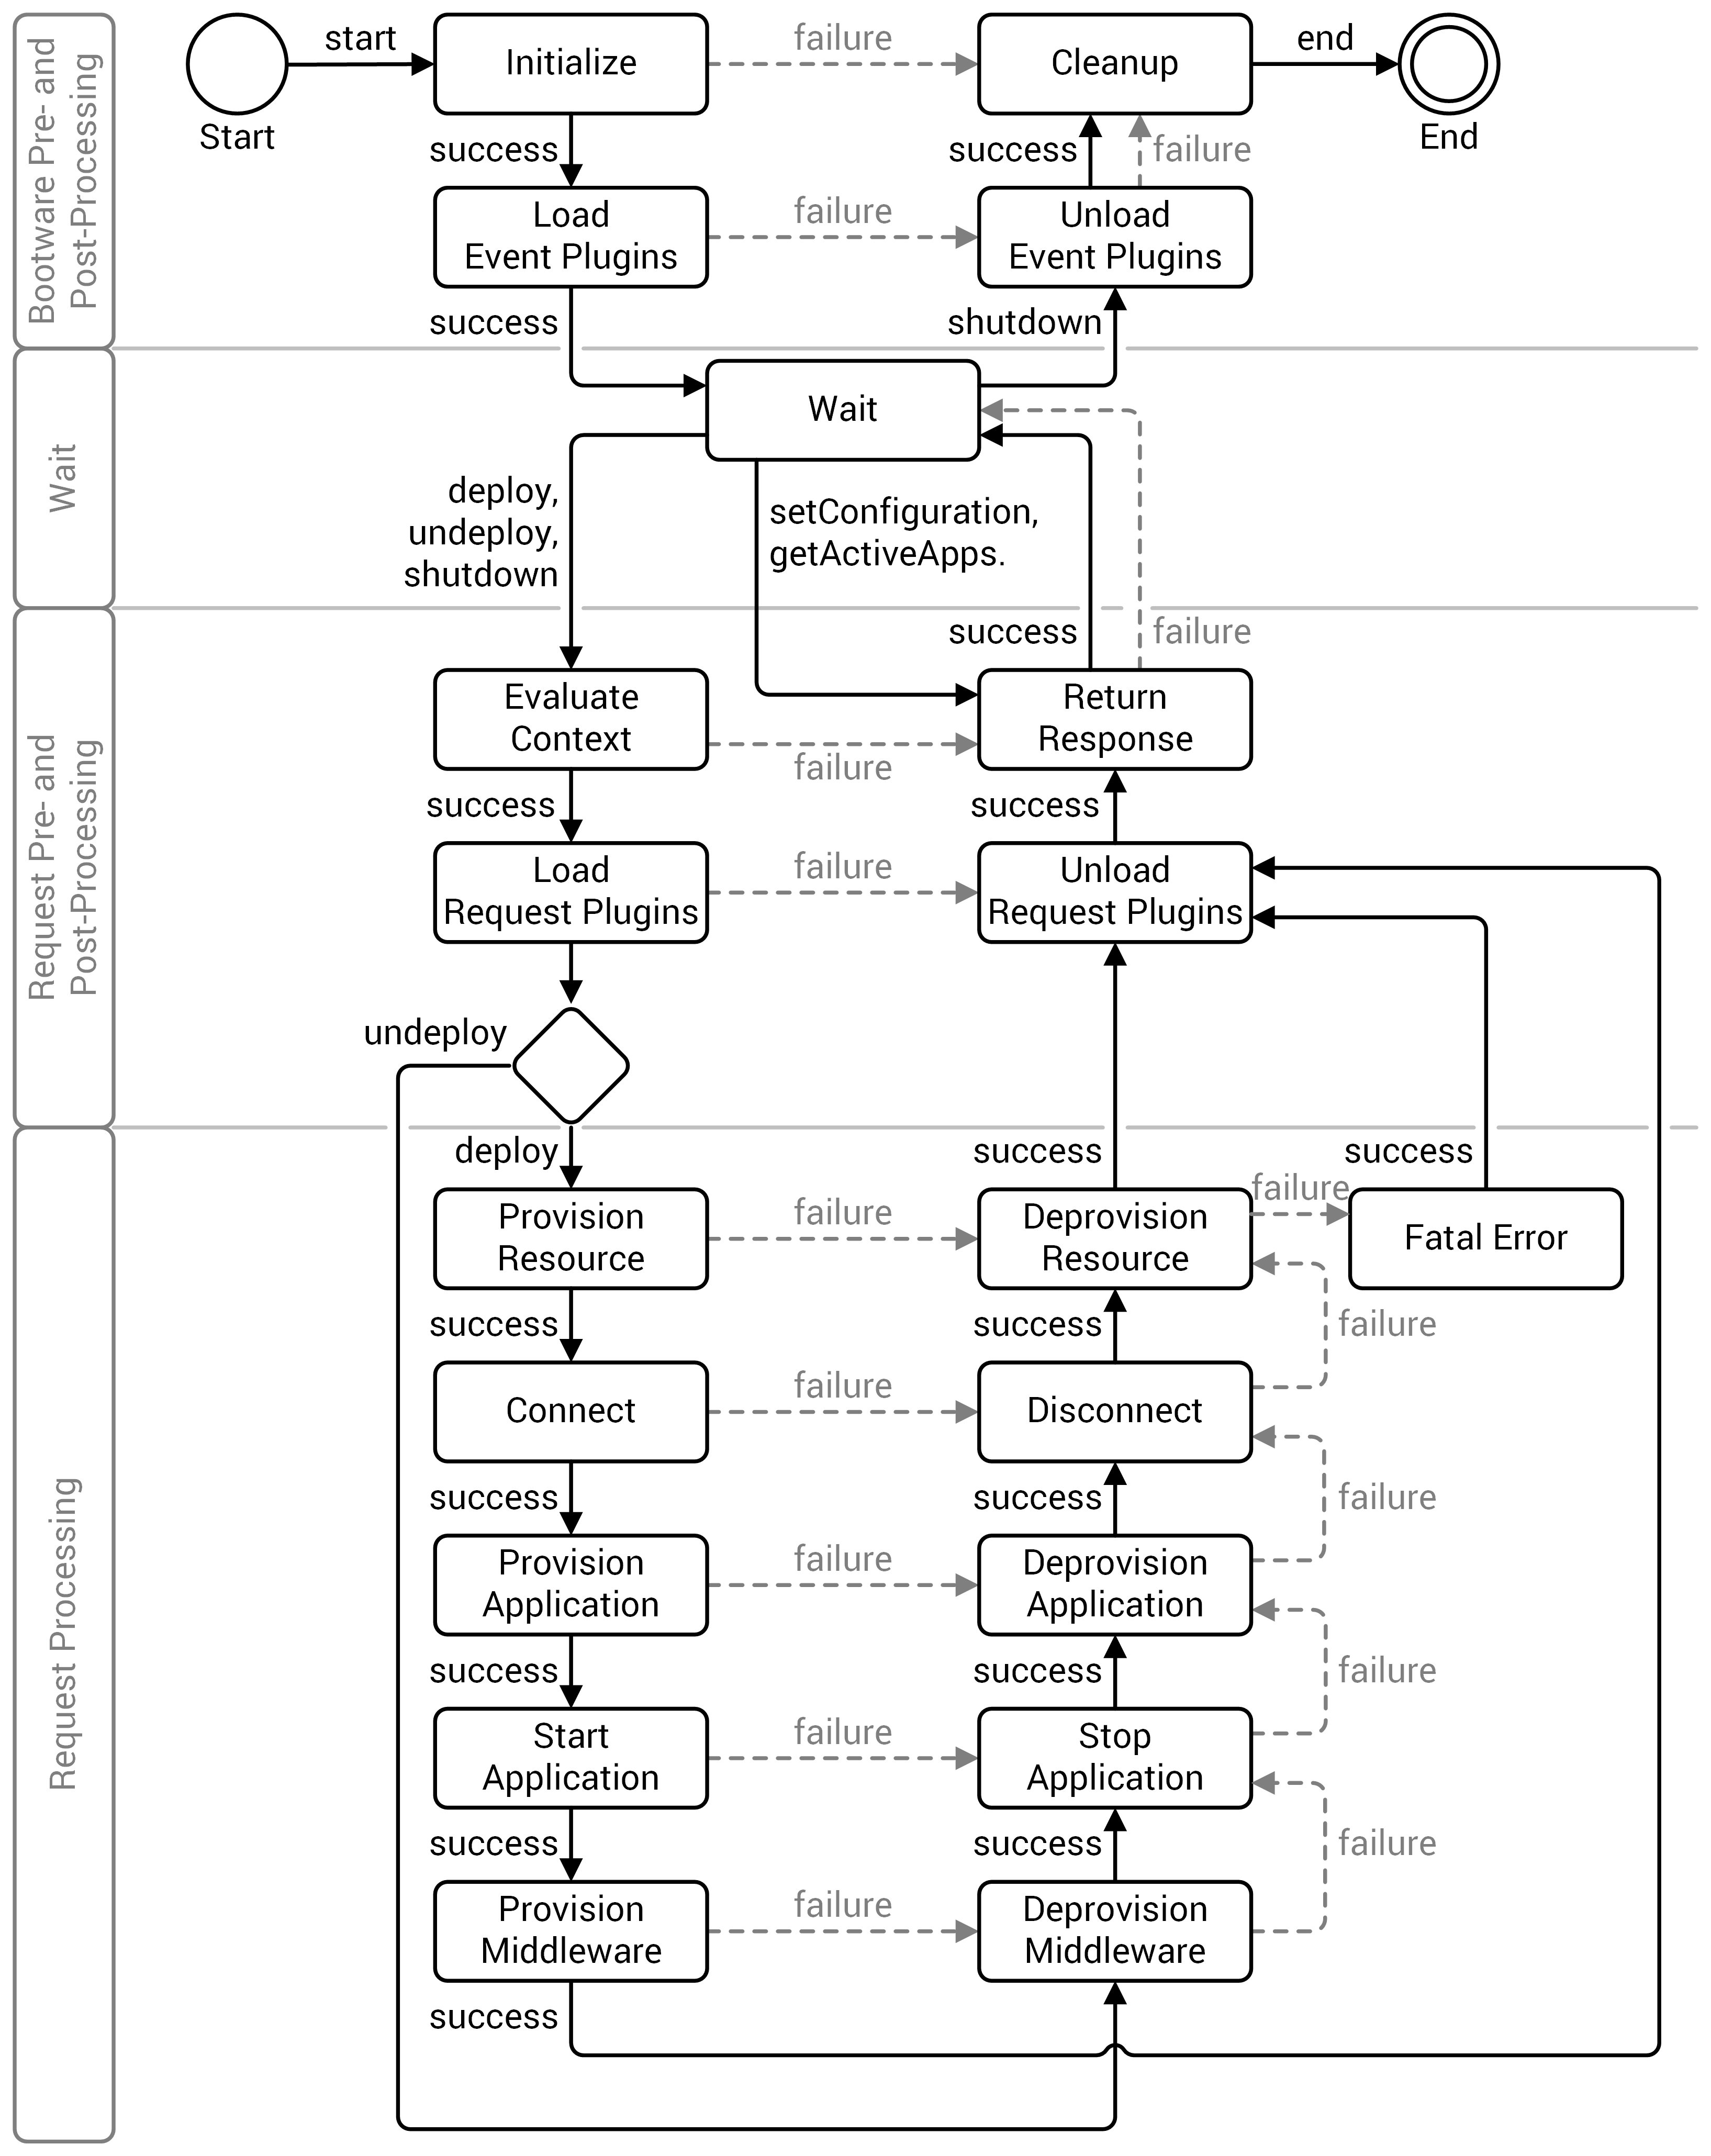
\includegraphics[resolution=600]{design/assets/flow_remote}
	\caption{Execution flow in the remote bootware.}
	\label{image:flow_remote}
\end{figure}

\pagebreak

Like the local bootware, the remote bootware went through the initialization steps shown at the top of \autoref{image:flow_remote} when it was started by the local bootware.
It then waited in the \textit{wait} activity for a request.
Now, it receives the request from the local bootware, creates the context, loads the request plugins and executes the deploy operation.
This should result in a provisioning engine being started by the application plugin.
After that, the remote bootware executes the new \textit{provision middleware} activity at the bottom left of \autoref{image:flow_remote}, which will use the just started provisioning engine to deploy the workflow middleware by executing the provision workflow middleware plugin.
Once the middleware is running, the remote bootware is finished with this request and returns the information list containing the endpoint references of the middleware in the response to the local bootware, before returning to the \textit{wait} activity.

This brings us back to \autoref{image:flow_local}, where the local bootware has now received the answer from the remote bootware in the \textit{send to remote} activity.
Now, the local bootware can finish its request by sending back a response to the bootware adapter, before returning to the \textit{wait} activity.
The local bootware is now done until it is time to undeploy the remote bootware.
Meanwhile, the bootware adapter starts the workflow execution on the middleware, during which multiple calls from the provisioning manager to the remote bootware will occur, which will each time trigger the deploy or undeploy process fragments shown at the bottom, or the getActiveApplications operation only hinted at in \autoref{image:flow_remote}.

As \autoref{image:flow_local}, \autoref{image:flow_remote} and the description above show, this is quite a complicated process with many conditional transition.
Using traditional programming methods like if/else blocks to implement this process would lead to a rather unwieldy and complicated construct with lots of nested if/else blocks.
Therefore, it could be advantageous to use other methods that are more fitting for this process.
As we already described the process as a directed graph, it would be ideal if we could take this whole graph and use it in the bootware.
Fortunately, this is possible by implementing the process using a finite state machine.

\subsection{Finite State Machine}

In theoretical computer science, a \nom{Finite State Machine}{FSM} is a formal, abstract model of computation "consisting of a set of states, a start state, an input alphabet, and a transition function that maps input symbols and current states to a next state. Computation begins in the start state with an input string. It changes to new states depending on the transition function"~\autocite{fsm}.
In this context, a state is the "condition of a finite state machine [...] at a certain time. Informally, the content of memory"~\autocite{state}.
The start state is therefore the initial condition of a FSM.
The alphabet is a "set of all possible symbols in an application. For instance, input characters used by a finite state machine, letters making up strings in a language, or symbols in a pattern element. In some cases, an alphabet may be infinite"~\autocite{alphabet}.
The transition function is a "function of the current state and input giving the next state of a finite state machine"~\autocite{transitionfn}.
FSMs can further be distinguished in deterministic and non-deterministic FSMs.
A deterministic FSM has at most one transition for each symbol and state, whereas a non-deterministic FSM can have non, one, or more transitions per symbol and state~\autocite{deterministic}.

Aside from its uses in theoretical computer science, FSMs also have practical applications in digital circuits, software applications, or as lexers in programming language compilers.
We are only interested in the use of FSMs for building software, so we can redefine what a FSM means for our case.
We want to use a FSM as an abstract machine that is defined by a finite list of states and some conditions that trigger transitions between those states.
Unlike a traditional FSM, we will not consume symbols from a set alphabet that will trigger state transitions.
We want the state transitions to be triggered by events that we can emit at any time, so we want an event-driven FSM.
The machine is in only one state at a time, its current state.
At the start of the machine execution, it will be in the start state.
From there, it can transition from one state to another when certain events are triggered, until it finally reaches an end state.
The states map directly onto the activities described in \autoref{image:flow_local} and \autoref{image:flow_remote}.
When The FSM enters a state, it executes a function associated with this state, which would be the implementation of said activities.
The result of the execution of this function determines to which state the FSM will transition next.
We will talk more about the actual implementation with FSMs in \autoref{implementation}.
